\documentclass{article}
\title{Power-Index Game Research Write-up 1}
\date{May 2018}
\author{Charlie Gerrie}
\usepackage[utf8]{inputenc}
\usepackage[english]{babel}
\usepackage{amsthm}
\usepackage{tikz}

\theoremstyle{plain}
\newtheorem{theorem}{Theorem}
\newtheorem{corollary}{Corollary}
\theoremstyle{definition}
\newtheorem{definition}{Definition}

\begin{document}
	\pagenumbering{gobble}
	\maketitle
	\newpage
	\tableofcontents
	\newpage
	\pagenumbering{arabic}
	\section{Behaviours}
		\subsection{Tesselation and Tauruses}
			\begin{definition}
				A pattern is a grid of tiles with specific sides. For example:
				\begin{itemize}
					\item
						a single weak tile
						\begin{figure}[h!]
							\begin{tikzpicture}
								\draw (0,0) rectangle (0.5,0.5);
							\end{tikzpicture}
						\end{figure}
					\item
						two strong tiles next to two weak ones
						\begin{figure}[h!]
							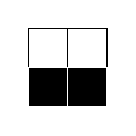
\begin{tikzpicture}
								\draw (0,0) rectangle (0.5,0.5);
								\draw(0.5,0) rectangle (1,0.5);
								\path[draw=white,fill=black] (0,-0.5) rectangle (0.5,0);
								\path[draw=white,fill=black] (0.5,-0.5) rectangle (1,0);
							\end{tikzpicture}
						\end{figure}
				\end{itemize} 
			\end{definition}
			\begin{definition}
				Congruence:
			\end{definition}
			\begin{theorem}
				\label{iteration}
				Tesselating a pattern in a dimension is the same as simulating
				that pattern individually on a cylinder looped in the dimension
				being tesselated, so long as the tesselation does not shear the
				pattern, and the border of the pattern is congruent for each
				element of the tesselation.
			\end{theorem}
			\paragraph{}
			Consider a pattern $\vec{p}$ being tesselated in a dimension, which
			we will take to be the vertical one. Observe that the number of
			vertices bordering the top of the pattern must equal the number of
			vertices bordering the bottom. Hence, let it have $n$ vertices
			$\{t_i : i \in [n]\}$ bordering its top, and $n$ vertices
			$\{b_i : i \in [n]\} $ bordering its bottom. Number these such that
			$t_i$ is in the same column as $b_i$.
			\paragraph{}
			Now consider the copy of
			$\vec{p}$ above $\vec{p}$, which we will denote $\vec{p}^a$, along
			with its top and bottom vertices $t^a_i$ and $b^a_i$.
			Since shearing is not involved in the tesselation, then $t_i$ will
			be connected to $b^a_i$. Similarly, the copy of $\vec{p}$ below,
			$\vec{p}^b$, has all its $t^b_i$ connected to $b_i$.
			\paragraph{}
			Observe that $t_i$, $t^a_i$, and all the other similarly indexed top
			vertices in the tesselation will be congruent. They will also all
			have congruent neighbors. 
			
			
			\begin{corollary}
				Tesselating a pattern in two dimensions is the same as
				simulating that pattern by itself on a taurus.
			\end{corollary}
		\subsection{1 and 2-movement}
			induction
		\subsection{Stability}
			stability, instability, and parastability. Pressure.
			The problem of environment and containment. 
	\section{The Periodic Table of Patterns}
		Describe the behaviour of several series of objects
		\subsection{Unstable Elements}
			\subsubsection{2-square}
			\subsubsection{even squares}
		\subsection{Parastable Elements}
		\subsection{Stable Elements}
			\subsubsection{odd squares}
			\subsubsection{chevrons}
				The odd case of chevrons
		\subsection{Tesselation-stable Elements}
			\subsubsection{1-stripes}
			\subsubsection{2-stripes}
			\subsubsection{1-squares}
			\subsubsection{2-squares}
	\section{Arbitrary Even Cycles}
		How to construct arbitrary even cycles in the power-index game
\end{document}